\chapter{Design}

Il presente capitolo descrive le scelte architetturali, tecnologiche e progettuali adottate per soddisfare gli obiettivi e i requisiti definiti nel capitolo precedente. L'attenzione si concentra sulle funzionalità sviluppate o analizzate durante il tirocinio, pur accennando alle linee guida per alcune delle funzionalità future, al fine di offrire una visione più completa del sistema.

La progettazione del nuovo sistema punta a superare i limiti identificati nel legacy, adottando un'architettura moderna, modulare e scalabile, che semplifichi la gestione e consenta l'integrazione di nuove funzionalità. Particolare attenzione è stata dedicata alla separazione delle responsabilità tra i vari componenti, alla progettazione di un backend flessibile e robusto agli errori, e alla realizzazione di un frontend intuitivo e con un aspetto enterprise.

Il capitolo è strutturato come segue: dopo una descrizione dell’architettura generale del sistema, si approfondiranno le principali componenti e funzionalità chiave, come la multiutenza e la gestione degli errori. Infine, saranno discussi gli aspetti relativi al miglioramento del database e alle strategie messe in campo per garantire una corretta migrazione dei dati dal sistema legacy.

\section{Architettura generale} Per la progettazione del nuovo sistema è stata adottata un'architettura a microservizi, caratterizzata da una separazione netta tra frontend e backend. Questa scelta è motivata dalla necessità di superare i limiti architetturali del sistema legacy, introducendo modularità e una chiara separazione delle responsabilità tra i vari componenti.

Nel nuovo sistema, il frontend è rappresentato da un singolo microservizio dedicato alla logica di presentazione dei dati e all'interazione con l'utente. Il backend, invece, è stato suddiviso in molteplici microservizi indipendenti, ciascuno dedicato a un modulo o a una funzionalità specifica dell'applicativo. Questa scomposizione consente di ottenere una maggiore flessibilità, facilitando sia l'aggiunta di nuove funzionalità che la manutenzione del sistema.

I microservizi comunicano tra loro utilizzando il protocollo HTTP e, più specificamente, attraverso le API RESTful che ciascuno di essi espone. Esse vengono inoltre utilizzate sia dal frontend sia per la creazione delle API pubbliche aziendali. Queste ultime, già presenti insieme al sistema legacy, sono state rinnovate per adattarsi alle nuove logiche di funzionamento introdotte nel nuovo sistema.

Una rappresentazione schematica dell'architettura del sistema è riportata in \Cref{fig:system-architecture}, dove sono evidenziate le principali componenti del frontend e del backend. Il diagramma mostra come il primo gestisca l'interazione con l'utente attraverso moduli specifici per il routing e per la gestione dello stato e della sessione, mentre il secondo sia organizzato in servizi dedicati a funzionalità come gestione utenti e autenticazione.

\begin{figure}
  \centering
  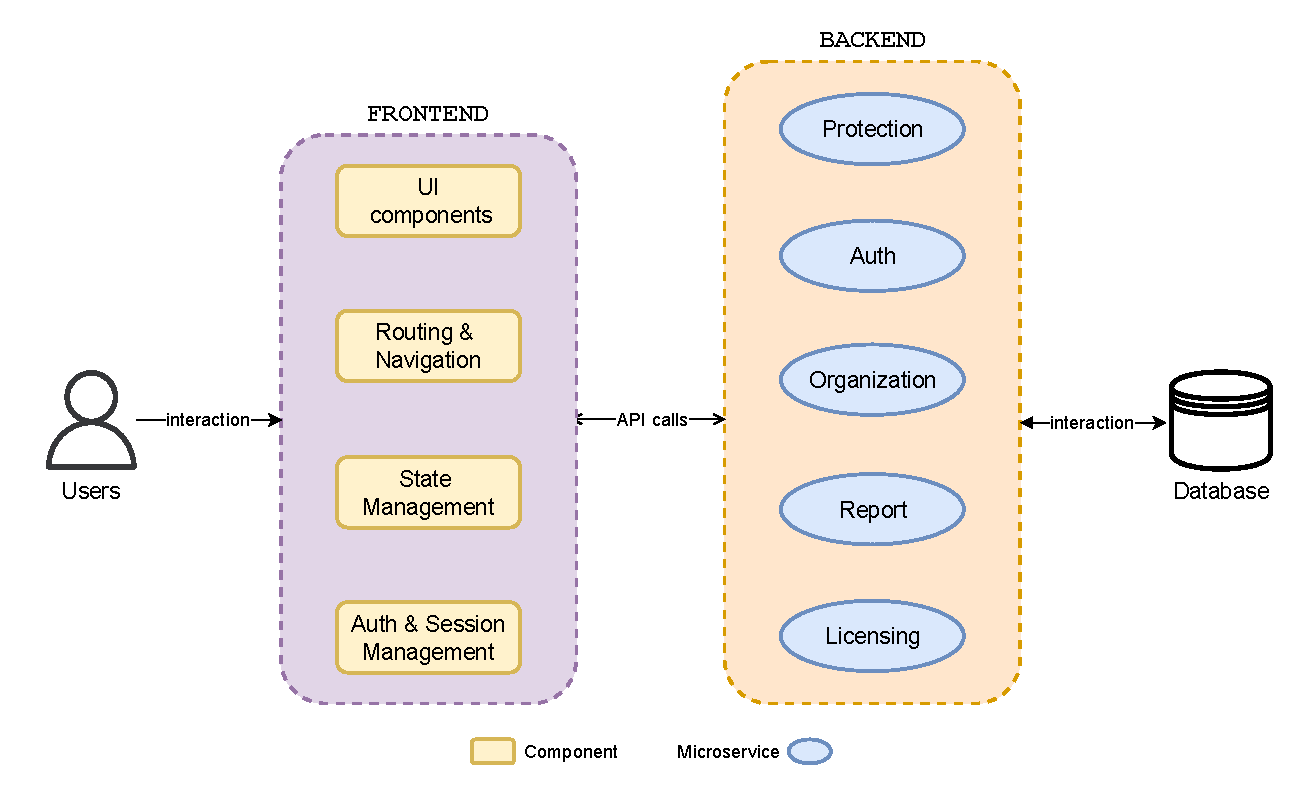
\includegraphics[width=1\textwidth]{figures/system-architecture.pdf}
  \caption{Architettura generale del sistema.}
  \label{fig:system-architecture}
\end{figure}

\subsection{Frontend}
Il frontend è stato progettato come una Single-Page Application (SPA), scelta che consente di offrire agli utenti un'esperienza fluida ed un accesso rapido da qualsiasi browser, senza bisogno di installare nessun applicativo. Questo microservizio si occupa esclusivamente della logica di presentazione, implementando l'interfaccia grafica e gestendo l'interazione con gli utenti finali. Infatti, tutte le operazioni di elaborazione dei dati, come le computazioni o la gestione delle regole di business, sono demandate al backend.

L'architettura del frontend segue un approccio modulare, in cui ogni pagina e componente è organizzato secondo una struttura gerarchica. Ciò consente di mantenere l'architettura chiara e scalabile, facilitando l'estensione del sistema e la gestione delle singole sezioni dell'applicazione.

Per garantire un design coerente e accelerare lo sviluppo dell'interfaccia, è stato adottato un template grafico altamente personalizzabile. Questo approccio ha consentito di ridurre i tempi di progettazione dell’UI, mantenendo al contempo la flessibilità necessaria per adattare l’aspetto grafico alle esigenze specifiche del progetto.

\subsection{Backend}
Come già accennato, il backend non è stato concepito come un unico servizio monolitico, ma si è optato per una suddivisione in più microservizi, ciascuno responsabile di una specifica funzionalità o modulo del sistema. La definizione di questi microservizi è stata guidata dall'analisi del dominio (\Cref{sec:domain-analysis}), individuando le principali entità e le loro responsabilità all'interno dell'architettura complessiva. Questo approccio ha permesso di modellare il backend in modo coerente con le esigenze del sistema, garantendo una chiara separazione delle responsabilità e facilitando l'evoluzione futura della piattaforma.

Di seguito, vengono descritti i principali microservizi di cui il backend è composto:
\paragraph{Auth}
Il microservizio \texttt{auth} è responsabile dell'autenticazione e dell'autorizzazione degli utenti. L'autenticazione è implementata attraverso il meccanismo JWT (JSON Web Token), che consente di gestire sessioni sicure senza la necessità di mantenere uno stato lato server.
L'autorizzazione, invece, fornisce un sistema per determinare se un utente ha i permessi necessari per eseguire una determinata azione. Questa valutazione si basa sul ruolo dell'utente e sulla licenza a lui associata, garantendo così un controllo granulare sugli accessi alle funzionalità della piattaforma.

\paragraph{Report}
Il microservizio \texttt{report} gestisce la generazione e la visualizzazione dei report relativi alle attività di filtraggio DNS. Nella prima versione del sistema, questa funzionalità è limitata alla visualizzazione di report specifici per gli MSP. Questo microservizio si interfaccia con il database per raccogliere e aggregare i dati necessari, fornendo agli utenti una panoramica dettagliata sull'attività di filtraggio e sull'efficacia delle policy applicate.

\paragraph{Organization}
Il microservizio \texttt{organization} è un componente chiave per l'implementazione della multiutenza. Esso si occupa di gestire tutte le operazioni CRUD sugli utenti, consentendo di creare nuovi account, modificare i ruoli, nonché rimuovere utenti dalle organizzazioni.
Grazie a questo servizio, più utenti possono essere associati a un'unica organizzazione con livelli di accesso differenziati, migliorando la flessibilità e la gestione delle autorizzazioni.

\paragraph{Protection}
Il microservizio \texttt{protection} è responsabile della gestione delle policy di protezione applicate agli utenti e alle organizzazioni. Questo servizio permette di creare, modificare ed eliminare i profili di protezione, ossia insiemi di regole che determinano quali contenuti possono essere filtrati o consentiti.
Inoltre, gestisce la creazione e l’amministrazione dei profili condivisi, che consentono di applicare una configurazione comune a più clienti senza dover definire manualmente le stesse regole per ciascuno di essi.

\paragraph{Licensing}
Il microservizio \texttt{licensing} si occupa della gestione delle licenze associate agli utenti e alle organizzazioni. Attraverso questo servizio, è possibile visualizzare lo stato delle licenze attive, gestire le assegnazioni e monitorare la loro scadenza.
Questo microservizio è essenziale per garantire che ogni utente abbia accesso solo alle funzionalità previste dal proprio piano, permettendo un controllo efficace sui livelli di servizio offerti.

\subsubsection{Architettura a livelli}
I microservizi appena discussi adottano un'architettura uniforme, basata sull'esposizione di API REST, garantendo una progettazione modulare e scalabile. Tale struttura consente di mantenere indipendenti le diverse componenti del sistema, facilitando la manutenzione e l'evoluzione del software. Ogni microservizio è organizzato in più livelli, ciascuno con responsabilità ben definite, come illustrato in \Cref{fig:microservice-architecture}:

\begin{itemize}
  \item \textbf{Routes}: rappresenta il punto di ingresso delle richieste HTTP. Questo livello si occupa di applicare eventuali middleware, come quello per la gestione dell'autenticazione JWT e di indirizzare le richieste verso il controller appropriato, in base al metodo HTTP e al percorso richiesto.

  \item \textbf{Controllers}: ricevono le richieste dai Routes, validano i parametri in ingresso e delegano l'elaborazione ai servizi applicativi. Una volta ottenuto il risultato, i controller generano la risposta HTTP da restituire al client.

  \item \textbf{Services}: costituiscono il livello di business logic, elaborando i dati e orchestrando le operazioni necessarie. Questo livello intermedio permette di mantenere separata la logica di dominio dall'accesso ai dati, garantendo maggiore modularità e riusabilità del codice.

  \item \textbf{Repositories}: forniscono un'interfaccia per l'accesso ai dati, eseguendo operazioni di lettura e scrittura sul database. Questo livello è responsabile esclusivamente della gestione dei dati.

  \item Database: sebbene non sia parte integrante dell'architettura dei microservizi, rappresenta il livello di persistenza su cui vengono eseguite le operazioni di lettura e scrittura da parte dei Repository.
\end{itemize}

Questa suddivisione a livelli garantisce una chiara separazione delle responsabilità, migliorando la manutenibilità del codice e la scalabilità del sistema.

\begin{figure}
  \centering
  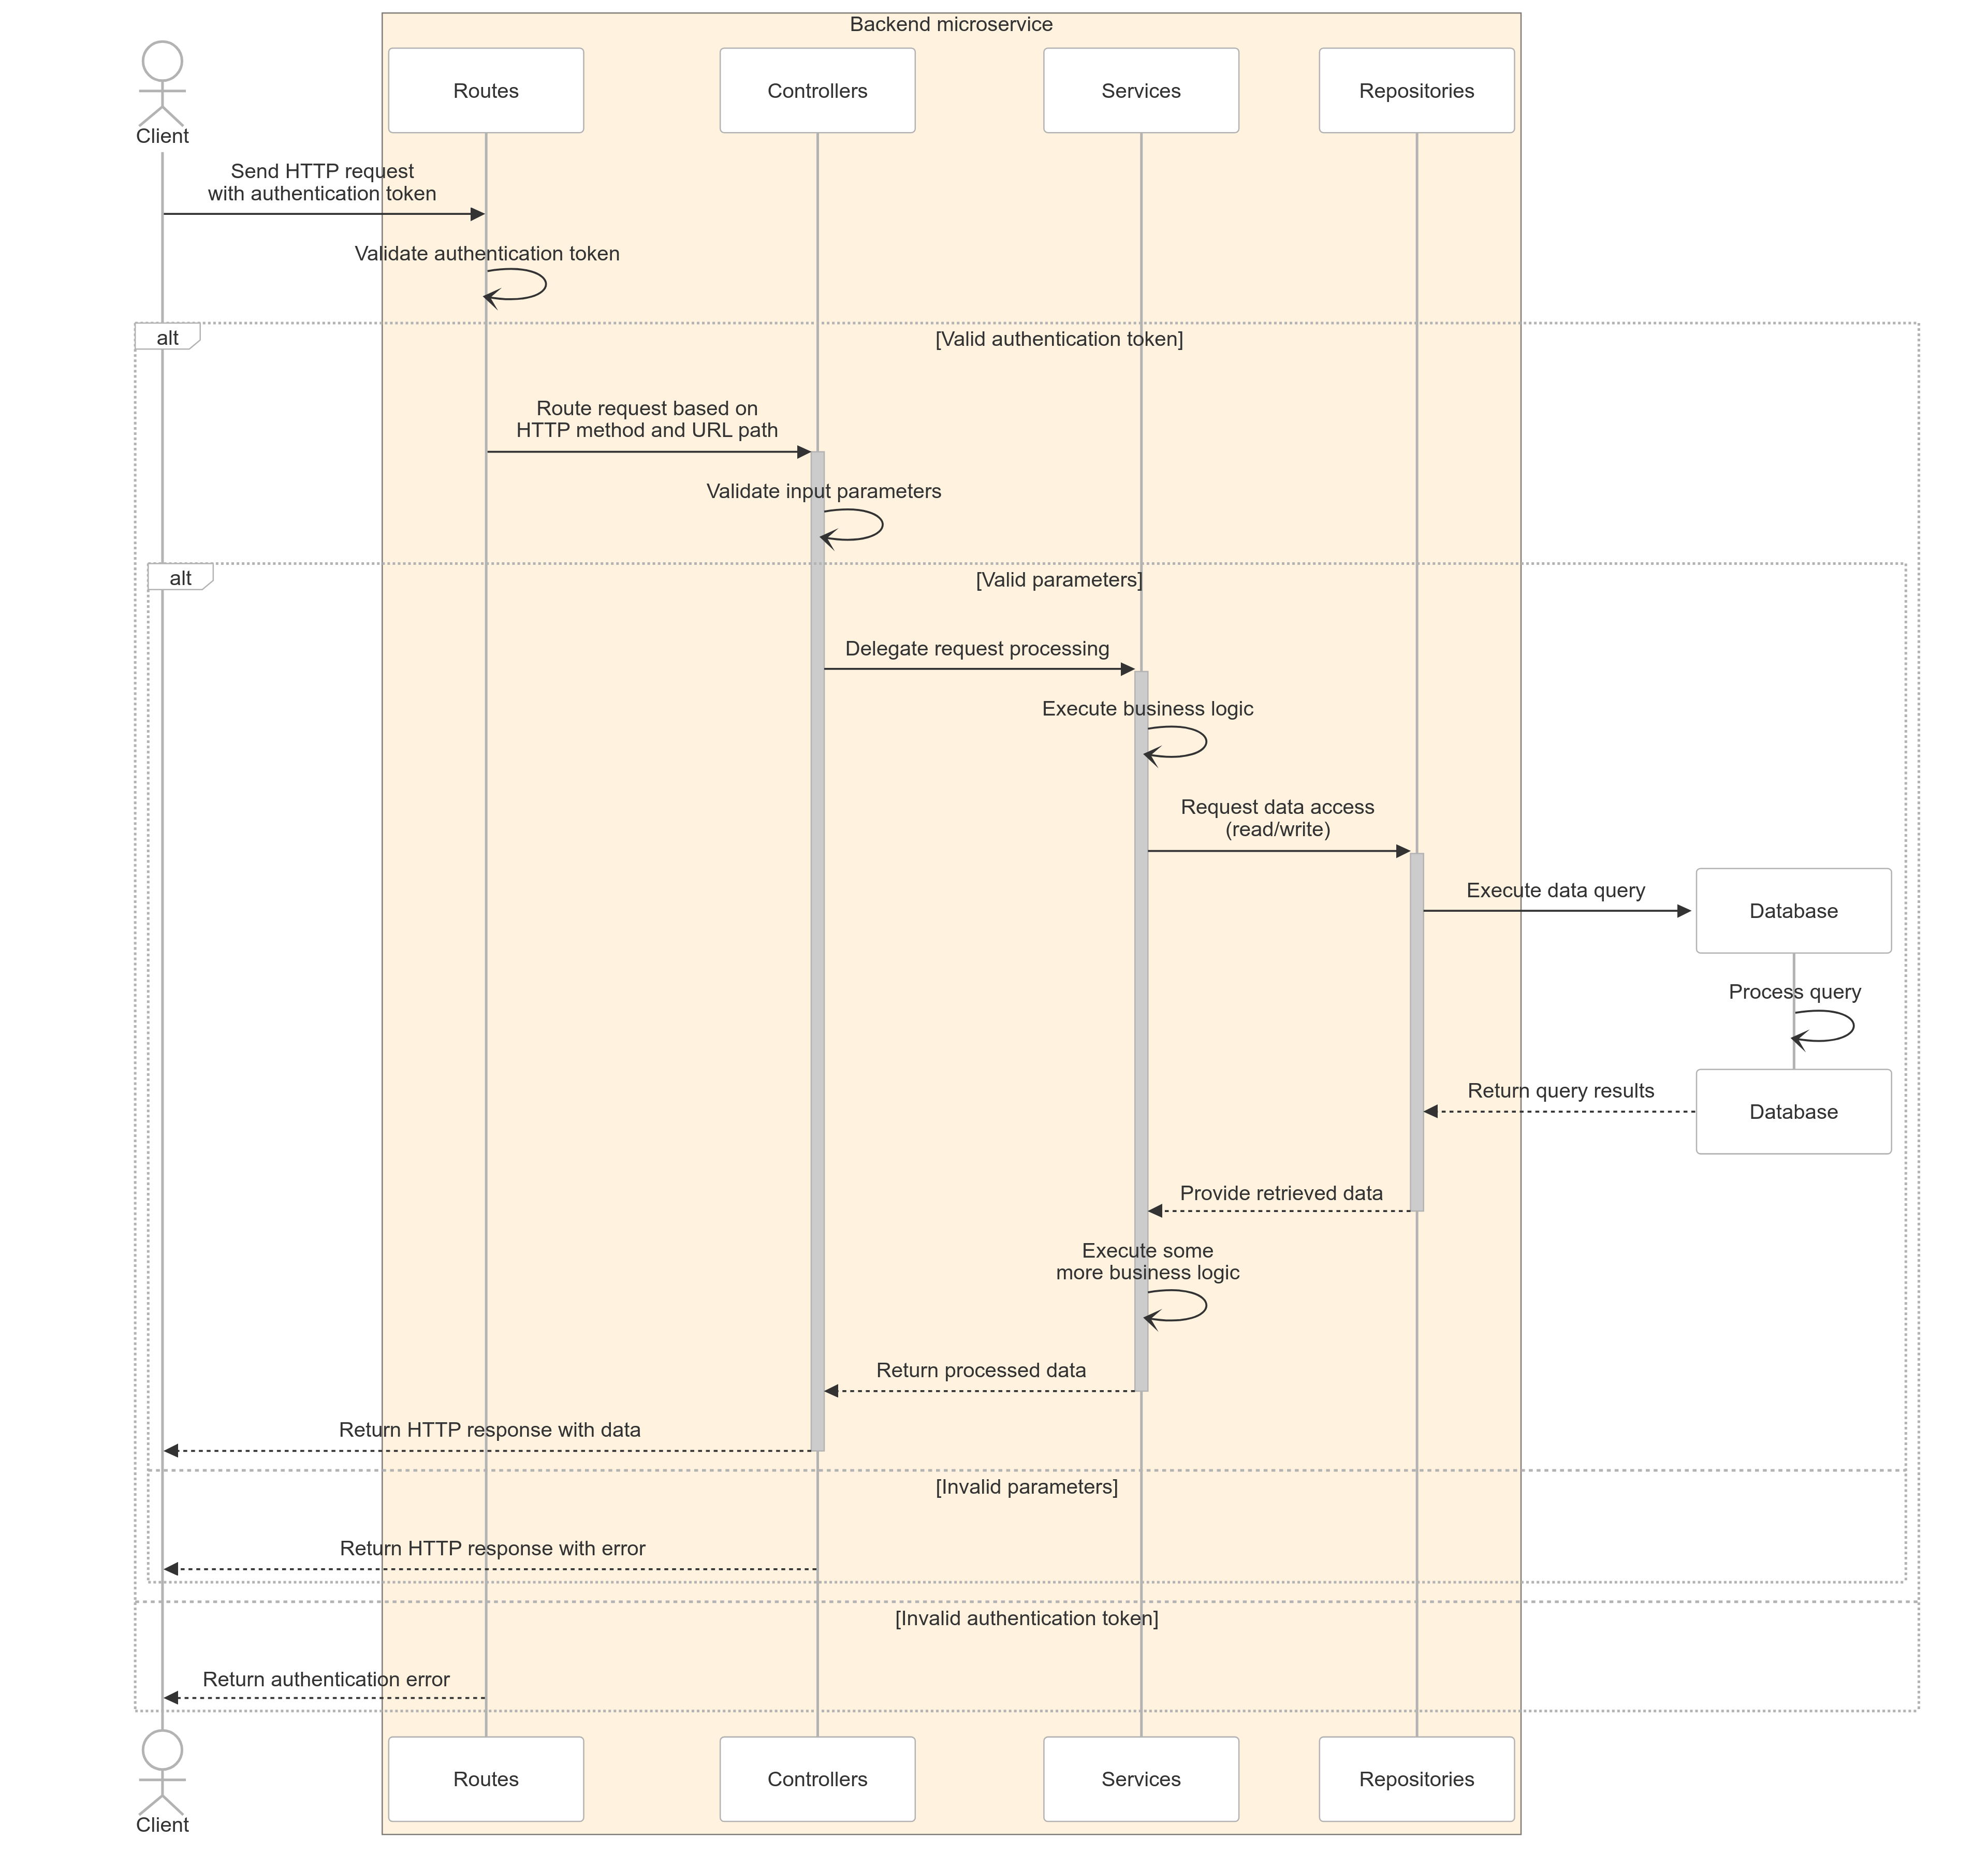
\includegraphics[width=1\textwidth]{figures/microservice-architecture.png}
  \caption{Diagramma di sequenza UML relativo all'architettura a livelli dei microservizi del backend.}
  \label{fig:microservice-architecture}
\end{figure}

Questa suddivisione in livelli garantisce una chiara separazione delle responsabilità, migliorando la manutenibilità e la scalabilità del sistema. Inoltre, consente di evolvere il backend in modo strutturato, rendendo più semplice l'aggiunta di nuove funzionalità o modifiche alle logiche applicative senza impattare gli altri componenti.

\subsection{Scelte tecnologiche}
Le tecnologie utilizzate per l'implementazione del nuovo sistema erano già state definite prima dell'inizio del presente contributo di tesi. Tuttavia, la loro adozione può essere motivata sulla base di considerazioni tecniche e di opportunità.

Per l'intero sistema, sia frontend che backend, è stato scelto il linguaggio TypeScript\footnote{\url{https://www.typescriptlang.org}}, che combina la flessibilità e la vasta disponibilità di librerie di JavaScript con i vantaggi di un linguaggio tipizzato. Grazie a TypeScript, è stato possibile sviluppare entità e funzionalità più robuste rispetto a un'implementazione in JavaScript puro, riducendo il rischio di errori a runtime. Il sistema di tipizzazione consente di individuare molteplici errori già in fase di compilazione, generando file JavaScript più affidabili e sicuri.

\subsubsection{Tecnologie del frontend}
Il frontend è stato sviluppato utilizzando Next.js\footnote{\url{https://nextjs.org}}, un framework basato su React. La scelta di React è stata dettata dalla volontà di mantenere la filosofia del sistema legacy, che forniva il pannello sotto forma di web application, e dalla sua combinazione tra ampia diffusione, efficienza e curva di apprendimento bilanciata. Tuttavia, piuttosto che utilizzare React in modo standalone, si è preferito adottare un framework che ne ottimizzasse l’utilizzo. Next.js è stato selezionato per le sue funzionalità avanzate, tra cui il pieno supporto a TypeScript e la gestione automatizzata di operazioni come il bundling e la compilazione, consentendo agli sviluppatori di concentrarsi sulla logica applicativa senza preoccuparsi della configurazione dell'ambiente di sviluppo.

Come strategia di routing delle pagine, si è scelto di utilizzare App Router\footnote{\url{https://nextjs.org/docs/app}}, il sistema di routing integrato in Next.js. Questo approccio permette di definire le rotte dell'applicazione in modo strutturato, organizzando il codice in base alla gerarchia delle directory. Inoltre, offre supporto per il rendering lato server, migliorando la flessibilità nella gestione e nel caricamento dei componenti.

Dal punto di vista grafico, la scelta del template TailAdmin\footnote{\url{https://tailadmin.com}} come base di partenza è stata motivata dalla sua somiglianza con il design desiderato per il nuovo sistema. La disponibilità di schermate predefinite e componenti riutilizzabili ha accelerato lo sviluppo dell’interfaccia, mentre la sua natura open source ha garantito massima flessibilità, permettendo modifiche e personalizzazioni senza vincoli.

\subsection{Tecnologie del backend}
Tutti i microservizi del backend utilizzano il framework Web Express\footnote{\url{https://expressjs.com}} per esporre le loro API REST. Questa scelta è stata dettata dalla leggerezza e rapidità del framework, oltre alla sua capacità di gestire le rotte in modo intuitivo e modulare. Express consente di definire una gerarchia di routing chiara, facilitando la suddivisione delle responsabilità tra i vari livelli dell'architettura. Inoltre, supporta l'integrazione di middleware personalizzati, aumentando la flessibilità nella gestione delle logiche applicative, come l'autenticazione e la validazione delle richieste.

Per i meccanismi di autenticazione, si è optato per un sistema basato su JSON Web Token\footnote{\url{https://datatracker.ietf.org/doc/html/rfc7519}} (JWT). Questa soluzione è ampiamente diffusa grazie alla sua semplicità di implementazione e alla possibilità di essere utilizzata in ambienti scalabili e distribuiti senza la necessità di mantenere uno stato centralizzato per le sessioni utente. A condizione che venga implementata correttamente, JWT garantisce un elevato livello di sicurezza, permettendo un controllo efficiente sugli accessi e l'integrazione con i microservizi in maniera indipendente.

Per quanto riguarda la gestione dell’accesso ai dati, si è scelto di adottare un ORM (Object-Relational Mapping) per semplificare l’interazione tra il backend e il database, evitando la necessità di scrivere manualmente query SQL complesse all’interno del codice applicativo. In particolare, la scelta è ricaduta su Prisma\footnote{\url{https://www.prisma.io}}, che si differenzia dagli Object-Relational Mapping tradizionali per il suo approccio dichiarativo. Più in dettaglio, a differenza degli ORM convenzionali, che mappano le tabelle del database su classi del linguaggio di programmazione, Prisma utilizza uno schema dichiarativo chiamato \textit{Prisma Schema} come unica fonte di verità per la struttura del database e dei modelli dell’applicazione. Questo consente una gestione più chiara e coerente dei dati, evitando le problematiche legate all'incompatibilità tra il modello a oggetti e quello relazionale.

Dal punto di vista della programmazione, Prisma fornisce una libreria lato client che permette di eseguire operazioni di lettura e scrittura sul database in modo tipizzato e sicuro, senza la necessità di gestire manualmente istanze di modelli complessi. Questo approccio offre numerosi vantaggi, tra cui:
\begin{itemize}
  \item \textbf{Maggiore coerenza tra codice e database}: le caratteristiche di Prisma Schema contribuiscono a semplificare l'evoluzione della struttura del database nel tempo, senza introdurre incongruenze o disallineamenti tra il codice e i dati.
  \item \textbf{Tipizzazione automatica}: grazie all’integrazione con TypeScript, Prisma garantisce che i dati manipolati nel codice rispettino sempre il formato atteso.
  \item \textbf{Query più intuitive e leggibili}: Prisma Client fornisce un'interfaccia semplice per eseguire operazioni CRUD, eliminando la necessità di scrivere query SQL complesse e riducendo il rischio di errori.
\end{itemize}
L'adozione di Prisma ha quindi reso la gestione del database più strutturata, sicura e manutenibile, migliorando la produttività nello sviluppo e garantendo una maggiore affidabilità nel trattamento dei dati.

\subsubsection{Scelte tecnologiche del database}
Il nuovo sistema adotta un database relazionale con tecnologia PostgreSQL, scelta dettata principalmente dalla necessità di garantire la compatibilità con i dati gestiti dal sistema legacy. Oltre a questo requisito, PostgreSQL è stato selezionato per le sue caratteristiche di affidabilità, scalabilità e performance, rendendolo una soluzione solida per applicazioni che devono gestire un elevato volume di dati e richieste concorrenti.

\section{Funzionalità chiave}
\subsection{Multiutenza e gestione degli utenti}
Nel nuovo sistema, la multiutenza si riferisce alla possibilità per un'organizzazione di disporre di molteplici credenziali di accesso, consentendo a diversi utenti di accedere al pannello di configurazione del filtro per amministrarne le caratteristiche o monitorare le statistiche, in base al loro ruolo. Questo rappresenta un notevole miglioramento rispetto al sistema precedente, in cui ogni cliente disponeva di un singolo account con permessi di amministratore. Tale limitazione risultava problematica in particolar modo per le organizzazioni più strutturate, che necessitavano di un accesso distribuito tra più figure con differenti livelli di autorizzazione.

\subsubsection{Modello attuale di gestione degli utenti}
Attualmente, come già spiegato nella \Cref{sec:domain-analysis}, gli utenti esistono solo nel contesto dell'organizzazione di cui fanno parte. Ogni organizzazione, infatti, al momento della creazione, dispone di un account utente con ruolo di amministratore (Admin). Quest'ultimo ha la possibilità di creare altri utenti, assegnando loro un ruolo specifico e un'organizzazione di appartenenza. Tale organizzazione può essere la stessa di chi effettua la creazione, oppure una delle organizzazioni gestite (nel caso di utenti appartenenti a MSP o Dealer). Inoltre, l'Admin può modificare le informazioni di qualsiasi utente della propria gerarchia, nonché eliminarlo.

\subsubsection{Gestione dell'autenticazione e della sessione}
L'autenticazione nel backend segue il meccanismo JWT, garantendo sicurezza e scalabilità nella gestione degli accessi. Le password degli utenti, prima di essere memorizzate nel database, vengono sottoposte a \textit{hashing} mediante la funzione \texttt{bcrypt}\footnote{\url{https://www.usenix.org/legacy/events/usenix99/provos/provos_html/index.html}}, utilizzando un ``fattore di lavoro'' pari a 10, che determina il numero di iterazioni dell'algoritmo e influisce sul tempo necessario per generare l'output. Questo parametro rende più oneroso il calcolo dell'\textit{hash}, ed il valore scelto aumenta la resistenza agli attacchi di forza bruta senza compromettere le prestazioni del sistema.

Durante il login, il backend genera e restituisce due token, in accordo con JWT: l'\textit{access token}, incluso nel corpo della risposta, e il \textit{refresh token}, inviato come cookie HTTP-only. Il primo incorpora le informazioni essenziali per l'identificazione dell'utente, tra cui il suo ID, l'email e il ruolo, permettendo al backend di verificare le autorizzazioni senza dover interrogare il database a ogni richiesta. Il secondo, invece, consente di ottenere un nuovo \textit{access token} senza costringere l'utente a eseguire nuovamente l'autenticazione, migliorando così l'esperienza d'uso.

Questa strategia non solo incrementa la sicurezza, evitando l’esposizione dei \textit{refresh token} nel codice lato client, ma semplifica anche la gestione per il frontend. Infatti, grazie all'uso dei cookie HTTP-only, il browser si occupa automaticamente dell'invio del \textit{refresh token} nelle richieste al backend, riducendo il rischio di furti di credenziali e migliorando la protezione complessiva del sistema.

\subsubsection{Limitazioni e aspetti da migliorare}
Il sistema non adotta ancora un modello completo di Role-Based Access Control (RBAC)\cite{DBLP:journals/compsec/Bertino03}, sebbene la sua architettura sia predisposta per supportarlo. Attualmente, sono previste solo due tipologie di utenti, Admin e ReadOnly, senza una distinzione effettiva nei permessi tra le due categorie. Gli utenti ReadOnly, infatti, possono eseguire le stesse operazioni degli Admin. Questa configurazione rappresenta una soluzione provvisoria, in attesa dell'implementazione di un sistema RBAC più strutturato. Una volta che esso verrà introdotto, gli utenti ReadOnly saranno limitati esclusivamente alla visualizzazione di report e statistiche, senza la possibilità di apportare modifiche.

Oltre alla gestione dei ruoli, un ulteriore livello di complessità deriva dal fatto che i permessi non dipendono esclusivamente dal ruolo assegnato all'utente, ma anche dai privilegi associati all’organizzazione di appartenenza, i quali a loro volta sono influenzati dalla tipologia di licenza in uso. Per affrontare questa complessità, è prevista l'implementazione di un sistema basato su una lista di permessi derivanti da questi fattori. Tali permessi verranno poi aggregati e consolidati dal backend durante il processo di autorizzazione, restituendo al client solo il fatto che l'utente abbia o meno il permesso di eseguire una determinata azione.

Questo sistema di permessi sarà applicato sia nel frontend, per regolare l'accesso alle pagine e ai componenti dell'interfaccia utente, sia nel backend, per proteggere le API e le operazioni disponibili per ciascun utente. In questo modo, sarà possibile garantire un accesso controllato e coerente su tutti i livelli del sistema, migliorando la sicurezza e l’affidabilità del processo di autorizzazione.

\subsection{Gestione degli errori}
Uno degli aspetti chiave della progettazione del nuovo sistema riguarda la definizione di un meccanismo di gestione degli errori strutturato e centralizzato. Questo sistema, sviluppato appositamente nell’ambito del tirocinio che ha portato alla presente tesi, consente di rappresentare e trattare in modo coerente le diverse tipologie di errore, garantendo uniformità tra backend e frontend e migliorando l’esperienza utente.

L'obiettivo principale di questa soluzione è evitare una gestione dispersiva e poco strutturata degli errori, introducendo un modello tipizzato e scalabile. Il sistema consente di differenziare gli errori in base al contesto e alla loro natura, assicurando che ogni anomalia sia rappresentata con un formato chiaro e prevedibile. Questo approccio consente inoltre di evitare l'esposizione di informazioni sensibili e di mantenere la logica di gestione degli errori separata dalle altre componenti del sistema.

\subsubsection{Gestione degli errori nel backend}
Il sistema di gestione degli errori nel backend è stato progettato attorno a una gerarchia di classi che permette di categorizzare le diverse tipologie di errore. Alla base vi è una classe astratta che definisce una struttura comune, fornendo un codice identificativo, un codice di stato HTTP e un eventuale insieme di dettagli aggiuntivi. Le classi derivate rappresentano errori specifici dell’applicazione e sono strutturate per coprire due aspetti principali: da un lato, scenari generici come accesso non autorizzato o errori interni del server; dall’altro, errori strettamente legati alle entità del dominio applicativo. In quest’ultimo caso, ogni entità è associata a una serie di errori tipici, come \texttt{UserNotFound} per indicare l’assenza di un utente richiesto o \texttt{UserCreateError} per segnalare un problema nella creazione di un nuovo utente.

Per mantenere un formato coerente, tutti gli errori seguono una mappatura predefinita, che associa ogni codice identificativo a un insieme strutturato di dettagli. Questa soluzione garantisce che ogni errore disponga delle informazioni necessarie per essere compreso dal frontend senza ambiguità. La gestione delle eccezioni è completata da un middleware centralizzato, che intercetta gli errori a tutti i livelli del backend e restituisce una risposta strutturata, includendo solo le informazioni rilevanti per il client.

Grazie a questa architettura, la gestione degli errori nel backend risulta modulare ed estensibile, permettendo di aggiungere nuove tipologie di errore senza impattare il resto del sistema.

\subsubsection{Gestione degli errori nel frontend}
Il sistema di gestione degli errori è stato progettato in modo da garantire una perfetta integrazione con il frontend. In particolare, il codice d'errore e i dettagli aggiuntivi forniti dal backend consentono al frontend di costruire messaggi chiari e contestualizzati per l'utente, senza che le stringhe siano \textit{hard-coded} nel backend.

Un aspetto rilevante della progettazione è la compatibilità con il sistema di multilingua del frontend. La struttura dei codici di errore, infatti, segue la stessa organizzazione delle directory utilizzate per la localizzazione delle stringhe, rendendo immediata la traduzione del messaggio in base alla lingua selezionata dall'utente. Questo permette di generare notifiche e avvisi coerenti senza necessità di duplicare la logica di gestione degli errori in più parti del sistema.

% \section{miglioramento del database}
% \subsection{Struttura del database}
% \subsection{Migrazione dei dati}
